I will focuse in this chapter on VR applications found in the literature for the visualization of bioinformatic data.

\section{Virtual Reality Chemical Space}
Virtual Reality Chemical Space is a VR application for the interactive exploartion of chemical space populated by Drugbank compounds\cite{drugbank}. It is also developed in Unity using C\# and the VRTK library. They use a particle system to render the particles of the chemical space. To render the particles, they use shaders instead of geometrical spheres as well, optimizing the number of vertices per datapoint in the scene. In order to reduce the motion sickness they have introduced a floor in the form of a grid acting as a static frame of reference. Also instead of letting the user move through the VR environment, they use a controller to move the point cloud. In Figure \ref{fig:drugbank} we can see an screenshot from the VR application. As we can notice in the screenshot, there is a subtle rendering of an outer space scene as an independent visual background. This is another technique to reduce the motion sickness that helps the user keep the notion of space. This is an interesting technique that we could have tried in BigNet VR.

They conclude in the article that the application that they have developed doesn't visualize an environment with an analogue in the real world, but instead a mathematical construct. Also some of the drawbacks that VR has compared to traditional solutions is that the VR headsets are not so comfortable as well as often-occurring eye strain and virtual reality sickness. They also conlcude that the application of VR in chemistry has more potential in the fields of education and training as for the current state of technology. The tools for chemistry need to be further evaluated wether they should be extended to VR.

\begin{figure}[h!]
    \centering%
    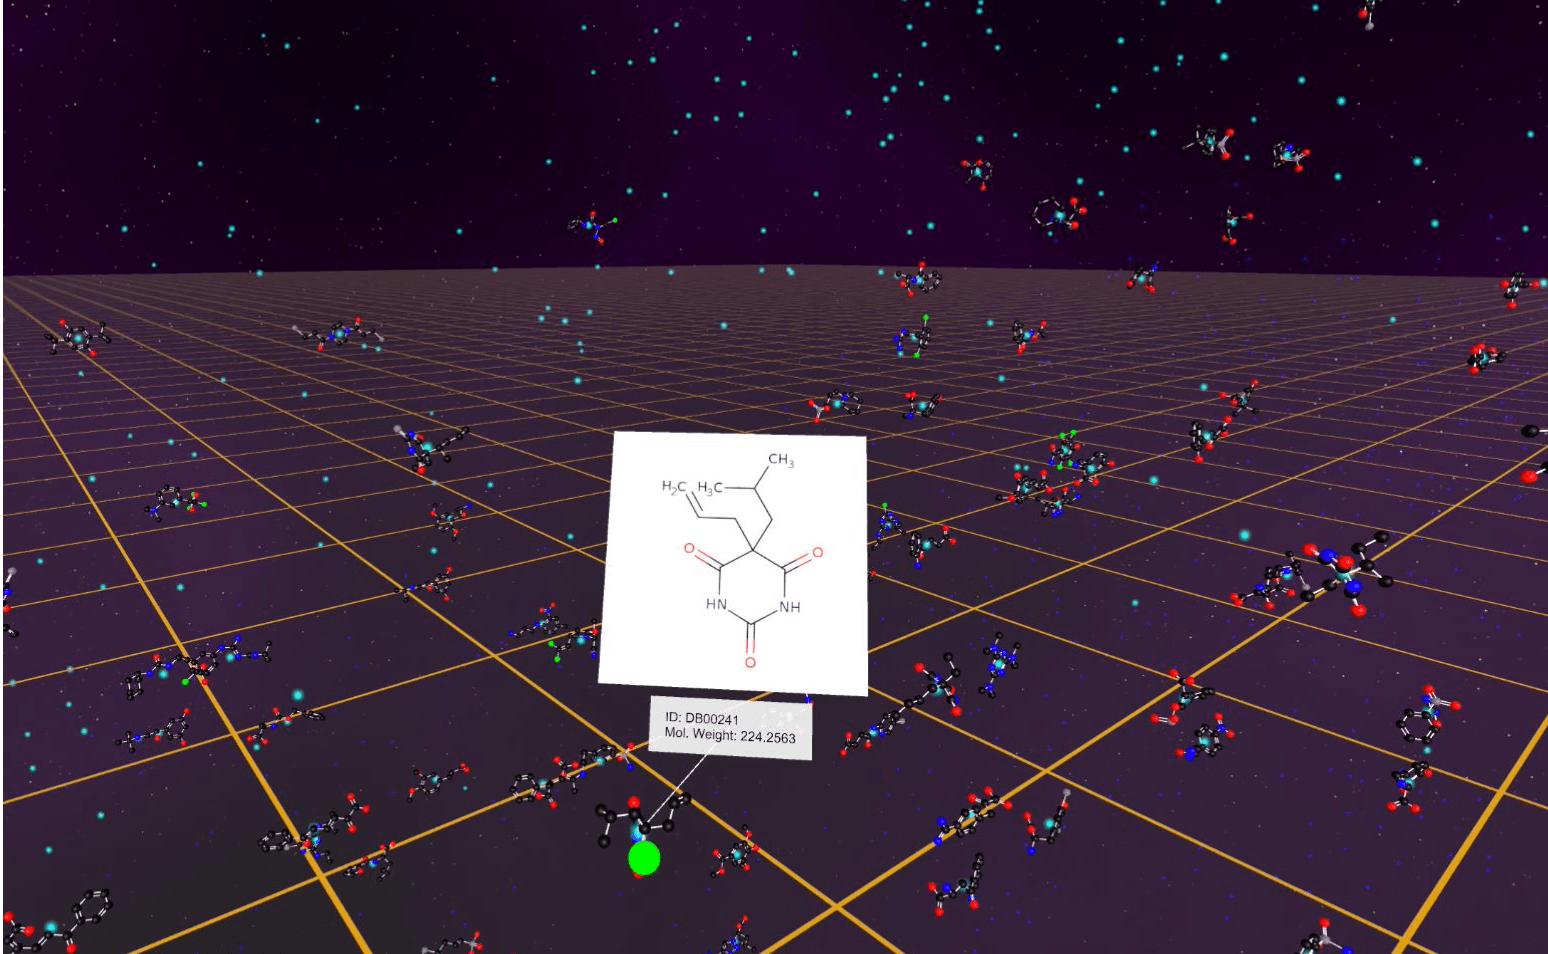
\includegraphics[width=\textwidth]{drugbank}
    \caption{Optimized virtual reality chemical space. Figure taken from \cite{drugbank}.}
    \label{fig:drugbank}
\end{figure}%

\section{BioVR}
BioVR is an interactive VR platform for integrated visual analysis of DNA/RNA protein structures\cite{biovr}. It is built in Unity and using C\#. The headset that they targeted the application to is Oculus Rift. One big difference between BioVR and our application is that in BioVR they use the hands for the interactions rather than the controllers. This can be very attractive and it could have worked very well for BigNet VR, since most of the interactions can be done with hand gestures. Also since early 2020, hand tracking has been integrated in Oculus Quest, making it easier for dveleopment\footnote{https://developer.oculus.com/documentation/unity/unity-handtracking}.
An screenshot of BioVR can be seen in Figure \ref{fig:biovr}. The user in BioVR can visualize the virtual hands in the virtual world and they are used for the interaction with the nucleotide sequence and UI menus. In BigNet VR instead of the hands we show the controllers, which help the user orientate in the space. The research concludes that using VR helps in create new workflows for researchers to view DNA/RNA sequence and protein structures. They also  of VR is that it is easy to integrate 2D user interfaces in the virtual world, as we can see in Figure \ref{fig:biovr} B.

\begin{figure}[h!]
    \centering%
    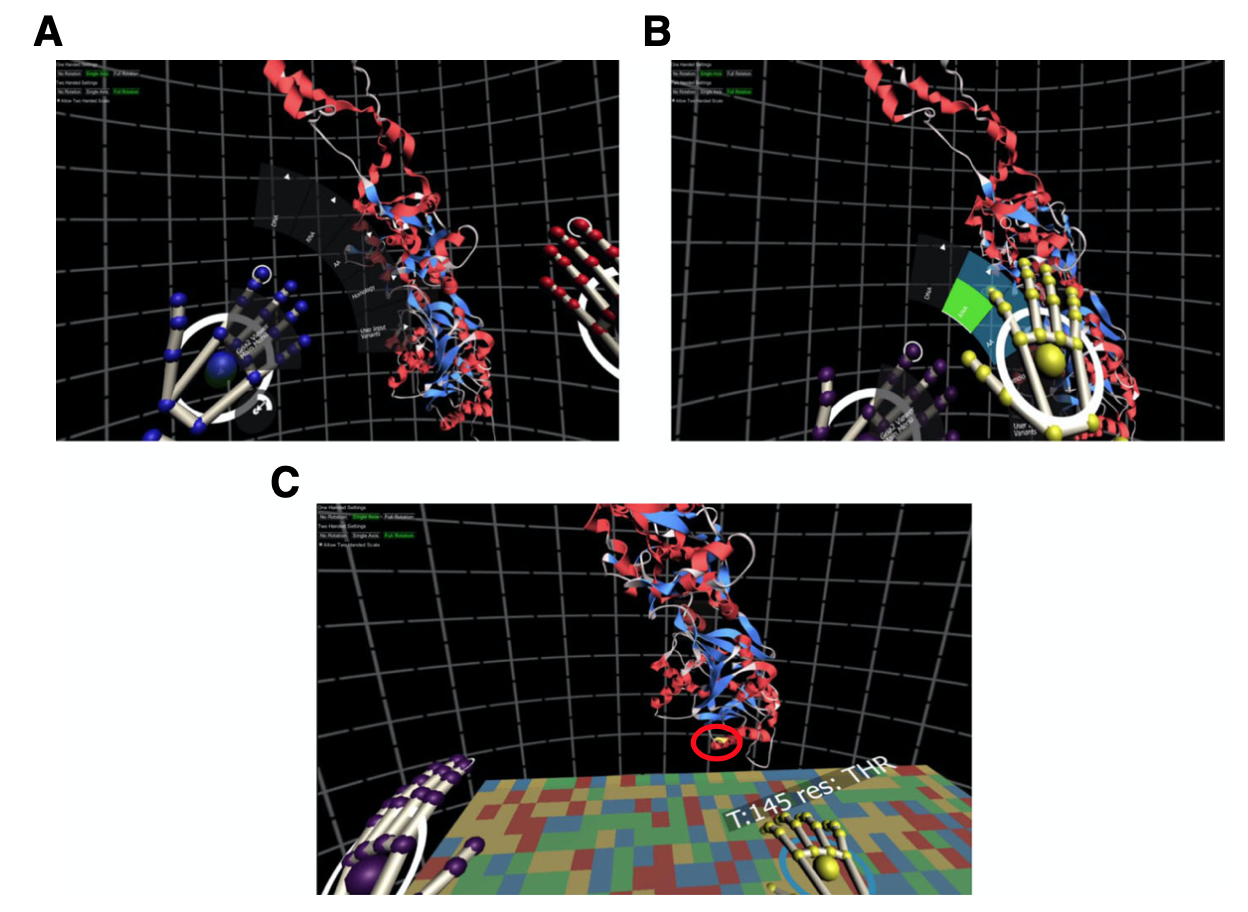
\includegraphics[width=\textwidth]{biovr}
    \caption{Screenshot from BioVR. Figure taken from \cite{biovr}.}
    \label{fig:biovr}
\end{figure}%

\section{CellexalVR}
CellexalVR is a virtual reality envirnoment for the visualization and analysis of single-cell RNAseq experiments that help researchers undertand their data\cite{cellexalvr}. The system is divided in two parts: the first one consists on the VR interface and the second is an R package called cellexalvrR that does back-end calculations and also provides functions that allows the user export the scRNAseq data from an R session for CellexalVR to read. CellexalVR was developed in Unity for HTC Vive (Pro). They used Unity and C\# and R for the implementation. They used libraries like VRTK, OpenVR and SteamVR as well in the implemenation.

Something that is interesting in CellexalVR is that it allows a multi-user mode via the Photon Unity Networking. This works sending information about the events to each user using Remote Procedure Calls. In Figure \ref{cellexavr} we can see an screenshot from CellexalVR where two users participate in the same session. Other users can also be in the same session but just be watchers and be in like a "ghost mode". This is something interesting that could be used in BigNet VR as well. Espcially the "ghost mode" could be useful so that other people can visualize the network at the same time from other perspectives.

\begin{figure}[h!]
    \centering%
    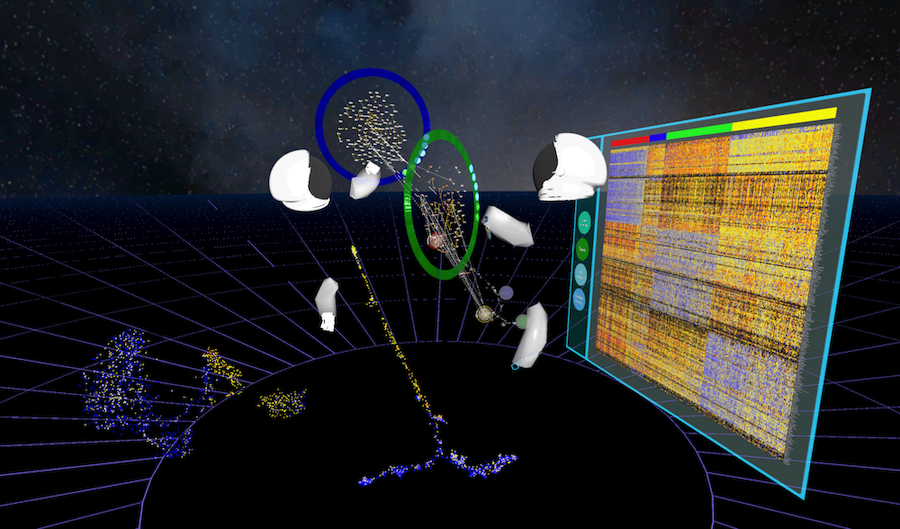
\includegraphics[width=\textwidth]{cellexavr}
    \caption{Screenshot from CellexalVR. Two users using CellexalVR at the same time. The head models were taken from NASA. Figure taken from \cite{cellexalvr}.}
    \label{fig:cellexavr}
\end{figure}%

\section{BigTop}
BigTop is a visualization framework in VR for the rendering of Manhattan plots in three dimensions\cite{bigtop}. Manhattan plots are usually 2-dimensionals, where genomic coordinates are displayed in the x-axis and the negative log-10 of the association P-value for each single nucleotide polymorphism (SNP) displayed on the Y-axis. Each dot on the Manhattan plot signifies a SNP then. In BigTop, the z-axis is used to display minor allele frequency of each SNP. This allows the identification of allelic variants of genes. As for the interaction, BigTop allows the user to select a node in order to obtain more information like the SNP name. BigTop is built in JavaScript with the React and A-Frame frameworks. It can also be rendered in any commercially available VR headsets and also in 2D web browsers.

The user in BigTop can move around by "walking" or use the keyboard if it is on the browser. 

\begin{figure}[h!]
    \centering%
    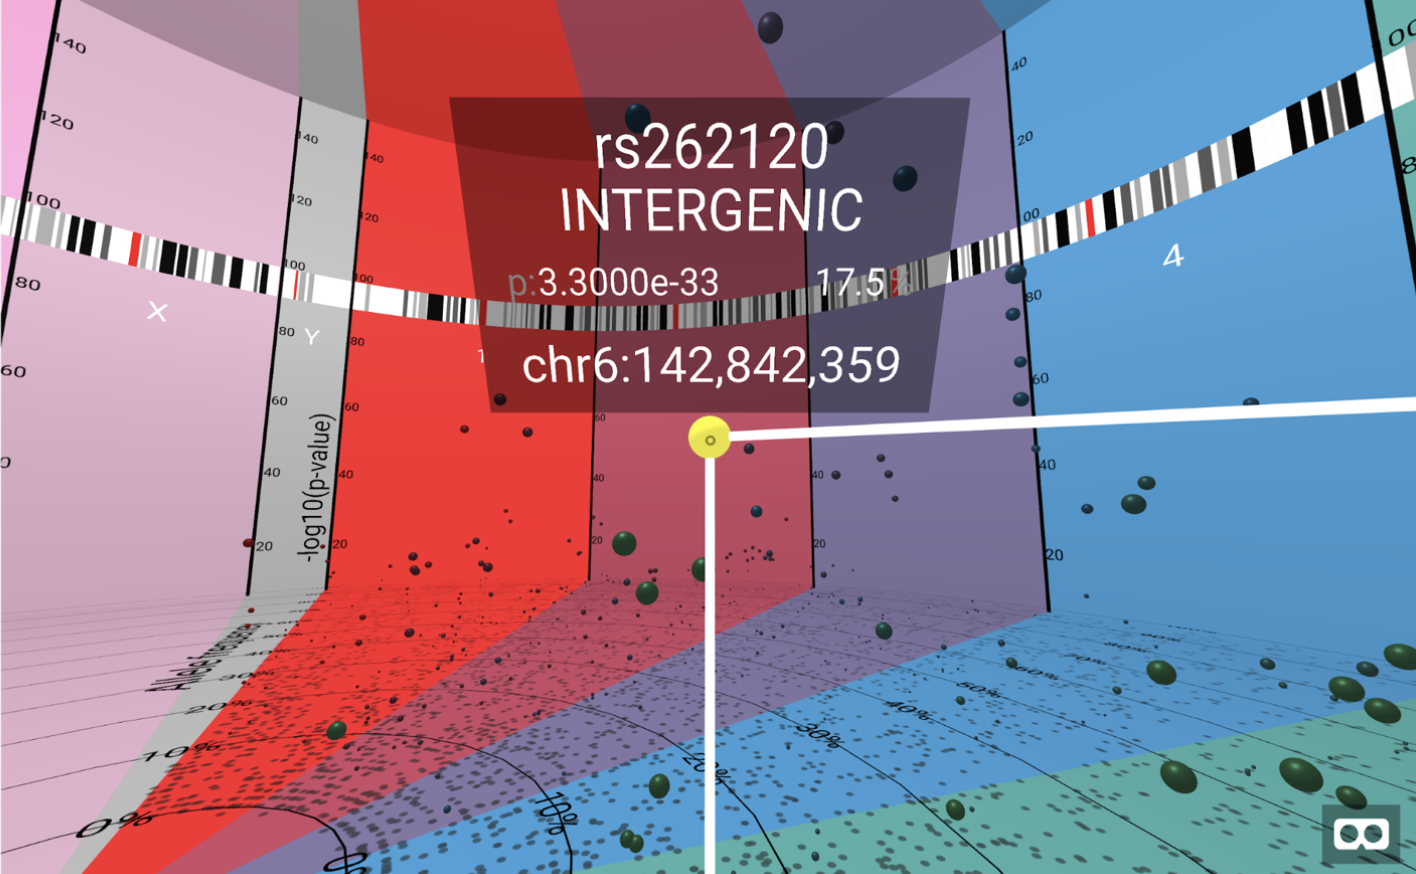
\includegraphics[width=\textwidth]{bigtop}
    \caption{Screenshot from BigTop. Figure taken from \cite{bigtop}.}
    \label{fig:bigtop}
\end{figure}%
